\documentclass{article}
\usepackage[utf8]{inputenc}
\usepackage[margin=0.5cm]{geometry}
\usepackage{graphicx}

\title{NEA - The Maze Game}
\author{Hugo Whittome}
\date{September 2020}
\begin{document}
    \maketitle
    \tableofcontents
    \clearpage
    \section{Analysis}
        \subsection{Overview}
            This is an exploration game, where you explore 5 levels of randomised mazes collecting items and followers on your way to help defeat the monsters.
        \subsection{Maze Generation}
            \subsubsection{Maze Needed}
                My plan for the maze is for it for it to be infinite, meaning that it only generates part of the maze at a time, and as you explore, you uncover more of the maze. However, for memory efficiency, the maze that is no longer loaded, won't be stored in memory and so deleted.
            \subsubsection{Types}
                There is both labyrinths and mazes. Labyrinths have only one path. This means that there is minimal choice in where the user can decide to go.
                The other type is mazes. These are multicursal, meaning it has multiple paths. This allows the user to choose their own path.
            \subsubsection{Approaches to Generation}
                \begin{itemize}
                    \item Cellular Automation Algorithm

                    This is based on John Conway's Game of Life, where a cell is created if it has exactly 3 neighbours and can survive it has 1-5 neighbors. However, this means that with the same starting pattern, the same maze will be created everytime.

                    \item Prim's Algorithm

                    This is where a random point on the maze is chosen as the starting point. Then all the surrounding areas are added to a list. Then the program continually generates new sections and adds more areas to the list, until the list is completely empty and all the spaces on the board is taken up. The positives with this is that it creates a randomised maze everytime, that takes up the whole map. However, the disadvantage is that when generating more sections, the maze cannot go back on itself.
                \end{itemize}
            \subsubsection{Conclusion}
                In conclusion, to make an infinite maze, I shall be using my own algorithm. This is slightly based off Prim's Algorithm, however instead of filling up the whole board, it leaves gaps. This is done by randomising entrances when placing a cell and then added only those possibilities to the list to generate more. This means that when the player moves north, it is able to generate paths that go back on itself however lead to dead end and not connect back up to the maze. This I feel will make a more dynamic maze when continually exploring the maze.
        \clearpage
        \subsection{Existing Solutions}
            \subsubsection{The Binding of Isaac}
                A similar game is The Binding of Isaac. What I liked about this game was the exploration and randomness, along with the challenge of fighting monsters in different rooms. However, I found it frustrating that there was limiting exploration on each level, as the level is not infinite. Furthermore, another issue I had was the only help that you could get was a familiar, in my game I wish to improve this by having set NPCs that you can find when exploring each level. Also, in binding of Isaac, the scrolling is  not smooth, jumping between each room. Also there are no corridors, making it seem less maze like.
                \begin{figure}[htbp]
                    \centerline{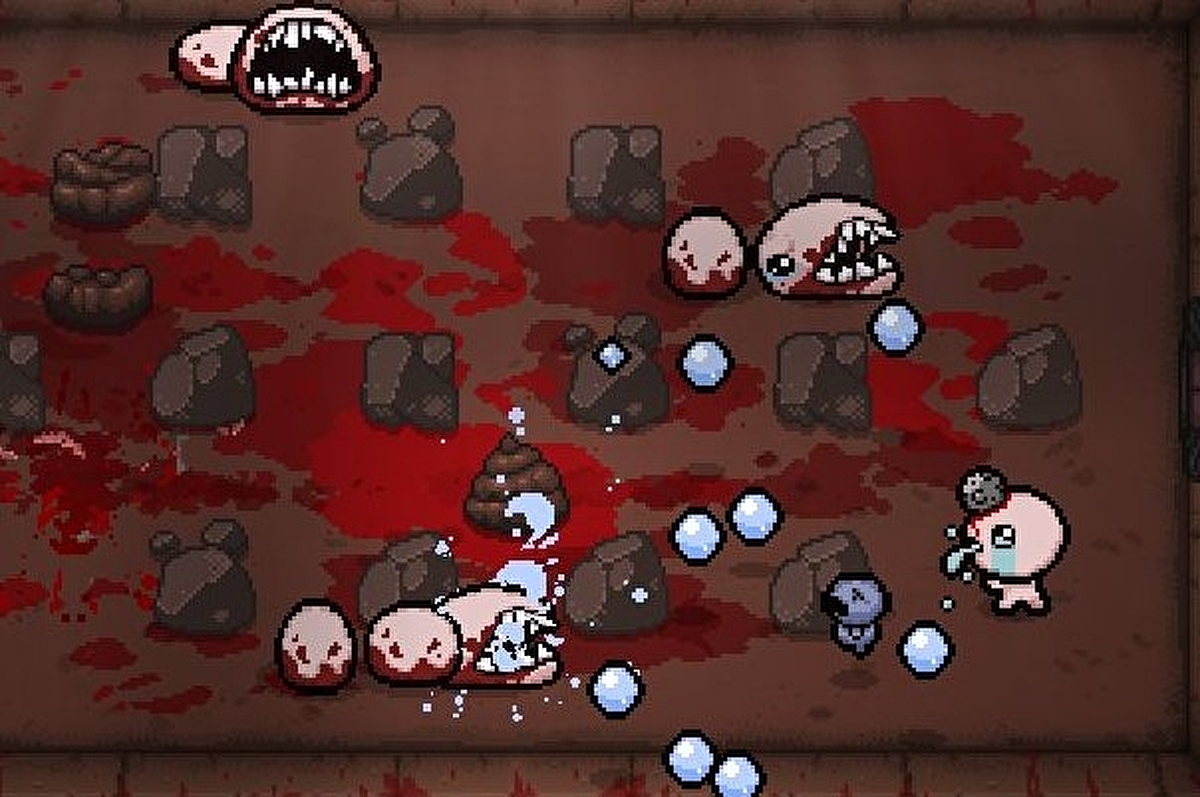
\includegraphics[scale=0.3]{img/The Binding of Isaac.jpg}}
                    \caption{Picture from the binding of Isaac, showing the player (bottom right) attacking the enemies}
                \end{figure}
        \subsection{End Users}
            \subsubsection{Description}
                Teenagers who enjoy exploration video games.
            \subsubsection{Questionnaire}
                \begin{itemize}
                    \item Have you played an exploration game before?
                    \begin{figure}[htbp]
                        \centerline{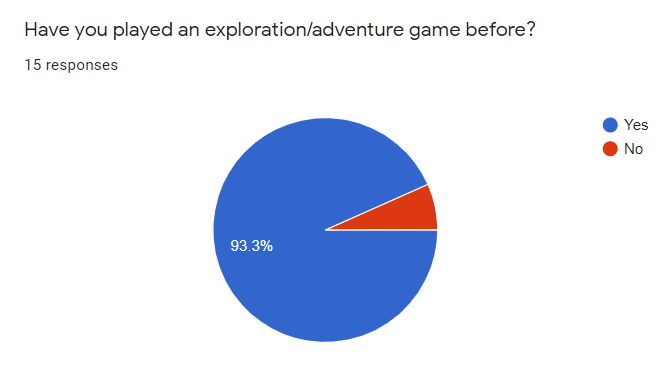
\includegraphics[scale=1]{img/Played Exploration Game.PNG}}
                        \caption{Responses from survey showing most people have played an exploration game}
                        \label{fig}
                    \end{figure}
                    \clearpage
                    \item How important is each section when looking for a game?
                    \begin{itemize}
                        \item Boss fights
                        \item NPCs that you can interact with
                        \item Enemies that attack you
                        \item Good story
                    \end{itemize}
                    \begin{figure}[htbp]
                        \centerline{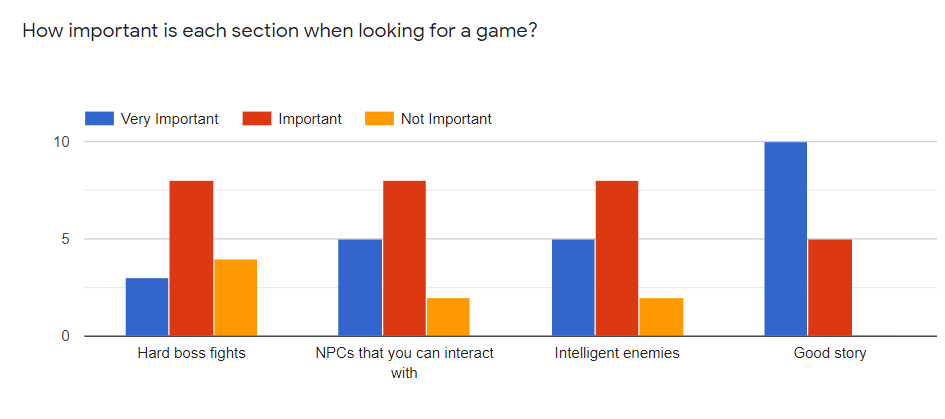
\includegraphics[scale=1]{img/Importance of games.PNG}}
                        \caption{Responses from survey showing that a good story is very important in a game}
                        \label{fig}
                    \end{figure}
                    \item What era do you like games to be designed as?
                    \begin{itemize}
                        \item Future
                        \item Modern
                        \item Medieval
                        \item Stone Age
                        \item Multiple eras
                    \end{itemize}
                    \begin{figure}[htbp]
                        \centerline{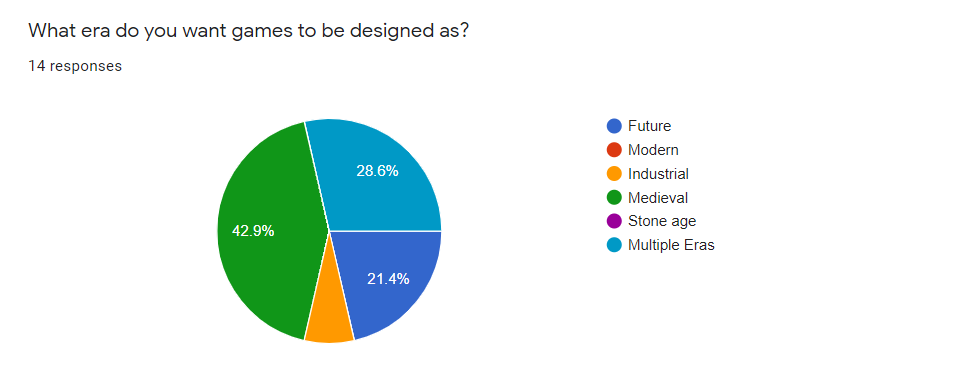
\includegraphics[scale=1]{img/Era of Games.PNG}}
                        \caption{Responses from survey showing that most people like a Medieval design}
                        \label{fig}
                    \end{figure}
                    \clearpage
                    \item Do you like games to have a story based ending or just a location to get to (e.g. flag at the end of Super Mario Bros Levels)?
                    \begin{figure}[htbp]
                        \centerline{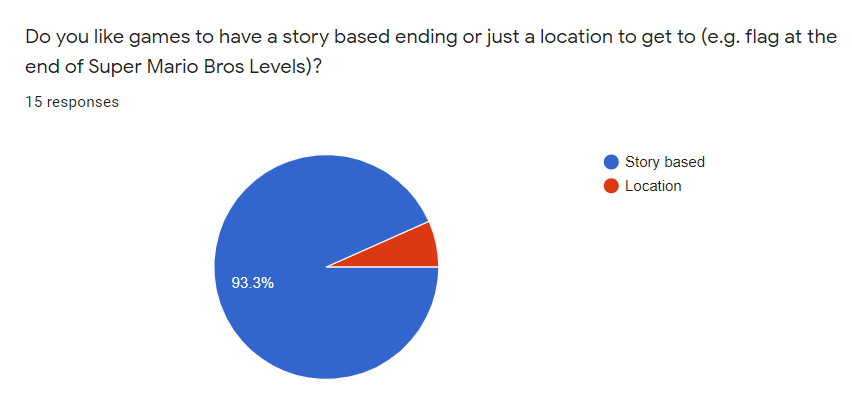
\includegraphics[scale=1]{img/Type of ending.PNG}}
                        \caption{Responses from survey showing the ending should be story driven and not just a point which the player has to get to}
                        \label{fig}
                    \end{figure}
                    \item Which do you prefer a weight-based system for the inventory (e.g. in Skyrim) or a space-based system (e.g. Minecraft)?
                    \begin{figure}[htbp]
                        \centerline{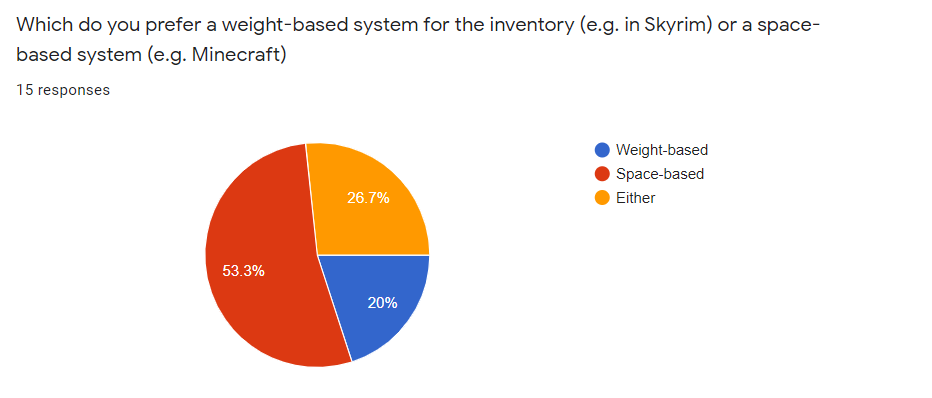
\includegraphics[scale=1]{img/Inventory system.PNG}}
                        \caption{Responses from survey showing that most people like a weight-based system in a game}
                        \label{fig}
                    \end{figure}
                    \clearpage
                    \item Do you prefer being able to move while attacking or a Pokémon style attack system?
                    \begin{figure}[htbp]
                        \centerline{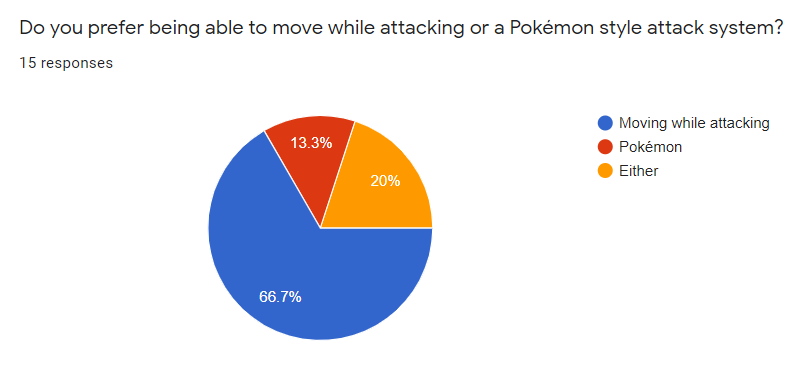
\includegraphics[scale=1]{img/Attacking System.PNG}}
                        \caption{Responses from survey showing that the attacking system should allow you to still control the player}
                        \label{fig}
                    \end{figure}
                    \item Have you played "The Binding of Isaac"?
                    \begin{figure}[htbp]
                        \centerline{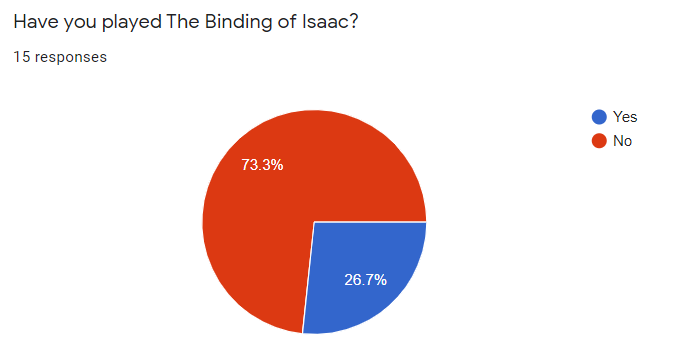
\includegraphics[scale=1]{img/Capture.PNG}}
                        \caption{Responses from survey showing that most people in this survey had not played The Binding of Isaac}
                        \label{fig}
                    \end{figure}
                    \begin{itemize}
                        \item If they had I asked what they liked about the game and what they think could be better (talked about in the conclusion)
                    \end{itemize}
                \end{itemize}
        \subsubsection{Conclusion}
            This research has made me prioritise the story as most people believed it to be very important in a game (as shown in \figurename{ 3}), this means that I will have to come up with a good story that gives an explanation to why the player is exploring a constantly changing maze. As an extension to this, it seems (as shown in \figurename{ 5}) that most people want a story-based ending, meaning that I will have to come up with an ending that suits the game. Furthermore, for the design, I will be going for a Medieval theme as it seems as though most people prefer that design scheme (as shown in \figurename{ 4}). Also, I have chosen to use a space-based system for the inventory as in \figurename{ 6}, most people responding that they prefer that system. Also, I will allow the player to attack at any point in the maze (for example shooting a projectile) because (as shown in \figurename{ 7}) people prefer it over an attacking GUI.

            As shown in \figurename{ 8}, only a few percentage had played The Binding of Isaac. when asked what they liked about the game, the responses included:
            \begin{itemize}
                \item The rougelike aspect (a subgenre of game that have generated levels, and tile-based graphics)
                \item The replayability and unique style
            \end{itemize}
            Most responses where talking about the rougelike aspect or the randomised levels. From this I have decided to use tile-based graphics with most sprites with a resolution of 64 pixels by 64 pixels to make it more rougelike also I want to make the maze as randomised as possible, meaning that many stats will be randomised.

            When asked what they would improve about the game, a few people responded saying:
            \begin{itemize}
                \item More routes down
                \item A good run is greatly depend on loot found in the first couple of floors.
            \end{itemize}
            From this, it seems that the reliance of chance for loot needs to be carefully managed. So, to combat this I have decided to change loot up between the levels, meaning that you cannot get overpowered loot on the first levels. Also I have decided to add a leveling system that allows you to upgrade your stats to allow more ways to play the game. Furthermore, I will need to create multiple ways to get down to different levels, for examples stairs, or a hidden passage that leads you to a treasure room on the next level.
        \subsection{Story}
            \subsubsection{Introduction}
                As seen from the questionnaire, it is very important for this game to have a good story. So this is the rouge outline of the story that I have planned for this game.
            \subsubsection{Background Infomation}
                In this world, there 5 five kingdoms (Ignius, Caelium, Ridiere, Regnio, Labyrinthius) listed below. Each live very differently with different beliefs and have different strengths. These kingdoms have a constant hostility and distrust towards one-another, which has resulted in many battles. The player's character will be the second born of Labyrinthius.

                Description of each kingdom:
                \begin{itemize}
                    \item \textbf{\emph{Ignius}} - A kingdom in the far south of the land. There kingdom is built ontop of the fire mountain, a volcano. This means that most of their buildings are black as they use the stone found around the volcano. Also, they use the lava found inside to build machinery. They use this volcano to through prisoners as a sacrifice to their god, Pozhar. They believe that Pozhar protects them from the wrath of the underworld, that is trying to escape and kill everyone.
                    \item \textbf{\emph{Caelium}} - A kingdom in the north of the land. Their capital is at the top of a mountain, looking down on the rest of the world. This has resulted them in seeing the other kingdoms below them. This resulted in them capturing people who wonder too far into their land, and using them as slaves. This has resulted in them using the slaves in wars, making their army extremely powerful. They worship the god who holds up the sky, Aakaash. They believe the god protects them from the sky falling onto them.
                    \item \textbf{\emph{Ridiere}} - A kingdom in the east of the land. The land around this kingdom is very flat, allowing them to farm a huge amount of crops. The capital is on a river, which allows transport of their crops to the other kingdoms. For this they worship the river, Flumen. The god who allows their crops to grow and deliver them into the mouths who need them. As the river washes away any bad deed, they believe in rehabilitation for their prisoners.
                    \item \textbf{\emph{Regnio}} - A kingdom in the west of the land. Known as being great builders. Their land is surrounded by rocky hills, in which they have built their kingdom on. Their defences are beyond anything any other kingdom has built. They do not believe in a god, instead believe in the power of mankind and they see people who believe in a god petty and weak. Their prisoners are treated with a punishment just of their crime, with time spend in a cage hidden below the ground.
                    \item \textbf{\emph{Labyrinthius}} - A kingdom in the center of all other kingdoms. A hub for trading and travellers, where many wizards reside as it's renounced for being a hub of knowledge. Their capital was founded around a whole in the ground, known as "de ore Dei" or the mouth of the god. The god is known as Kurtulmak, a living maze. One of the founders fell into the "de ore Dei" (a couple hundred years ago) and came out alive, talking of the wonders of this living maze and the monsters that lie beneath. They became known as a prophet and the only person to survive and be blessed by Kurtulmak. They have a tradition called "prophetam resurrectionem lesu Christi", where, when the second born of the monarch turns 15, they are chucked into the "de ore Dei", with one weapon of their choosing. If they are able to survive and escape the maze, they are blessed by Kurtulmak are crowned ruler over the kingdom before the first born.
                \end{itemize}

                Furthermore, throughout the map there are magical orbs, that once they have been put in staffs, that take hold of the power, allows the user to use the orb's power. These welders are called wizards, normally these wizards go out to try and discover more knowledge about these orbs to unlock their full potential. Then there are knights who own land in each kingdom and can be called by the king to come fight for him. These knights are usually very strong and have experience in battle. These people are usually quite aggressive and so have a bad view point around them, and most peasant try to avoid them to avoid conflicts that could result in their death, which has happened and some knights have been imprisoned for it - in the kingdoms in which this applies (all but Ridiere).

            \clearpage
            \subsubsection{NPCs}
                Throughout the game, the player will be able to find wondering NPCs, who were prisoners chucked down into the mouth to see if they could escape and be forgiven of all their crimes. The list of NPCs is as follows:
                \begin{itemize}
                    \item Max - A wizard from Labyrinthius, who was investigating how the maze moves. He was chosen to be the wizard to venture into the maze to look at it up close.
                    \item John - A pacifist from Ridiere, who was falsely accused of murder, and was chucked into the maze as a trial, if he survives, he will be declared innocent.
                    \item Cleo - A warrior from Ignius, wanting to prove herself as the best of the best.
                    \item Tabitha - Homeless servant from Labyrinthius sent down as a punishment for being caught stealing to survive.
                    \item Hope - A builder from Regnio who was admiring the entrance to the labyrinth when she fell in.
                    \item George - Merchant from Caelium who wanted to show that Caelium was better than every other kingdom, so he decided to jump in the entrance
                    \item Chayton
                    \item Emma
                    \item Simon
                \end{itemize}
            \subsubsection{Events}
                The player, the second born of the monarch, Leuok, has grown up knowing they will be chucked into the maze at 14, as part of the prophetam resurrectionem leu Christi tradition. This has caused the King to force them to train as hard as possible in combat and navigation without a map. Leuok has succeeded so far, and is extremely good with a sword and bow. The King, is torn up from this event as Leuok is his favourite child, and wants Leuok to succeed because the first born Ong, does not have the capability to be King. He is lazy and extremely selfish, two qualities that are not good for being King.

                After an introduction from a wizard, that is recording these events an unknown amount of years after the event, explaining everything in the previous paragraph, the player will be put into a temple that surrounds the whole. They will be given the choose of a one weapon before they go in. Once they have chosen, they will be told to jump into a hole, if they try to escape, they will be met with guards. The King will be seen, watching with a tear in his eyes, because he believes that Leuok will not survive.

                Once the player enters the whole, they will start to explore the maze, where they will fight monsters and maybe make friends will the NPCs that have been chucked in the whole previously. After a while of exploring, they will find a way down to the next level, where it will be taken back to the wizard recording the events, where he will interject saying "This is where Leuok found a way to the next stage, where the monsters were stronger, and fewer survived". This will repeat until the player reaches the 5th level.

                Once the player has reached the 5th level, they will be looking for the exit to outside (a set of stairs that leads to a door). Once they reached this door, they will be seen travelling through a corridor which will lead to an exit near the Ridiere kingdom. Then there will be a cut seen of Leuok being crowned ruler. The story will then end with the wizard ending it, as if it was the end of a great book.
        \subsection{Design Outline}
            \subsubsection{Classes}
                \begin{itemize}
                    \item Layer - This will allow the subclass to be stored as a layer and be updated and rendered by the application.
                    \item Level - This will store width and height of tiles and implement the A* algorithm for finding the shortest path between two roots.
                    \item Maze - This will store the rooms in a grid and implement the generation of the maze.
                    \item Camera - Generates the view matrix, that will allow the player to move around the map.
                    \item Entity - Stores x and y coordinates of an object in a given level.
                    \item Mob - Subclass of Entity, which implements a move function including collision detection.
                    \item Player - Stores the coordinates of the player.
                    \item Follower - Follows the player around and helps to attack the enemy.
                    \item Enemy - Attacks the player and their followers.
                    \item Item - Base class of all items that can be found throughout the maze.
                    \item Projectile - Is a projectile that travels in a single direction and then deals damage to a mob.
                    \item Room - This stores all the tiles
                    \item Tile - This will store a sprite with coordinates relative to the room.
                    \item Sprite - Stores every sprite that needs to be rendered during the game.
                \end{itemize}
            \subsubsection{Stats}
                Each stat will influence part of how you play the game. These will be upgraded through finding specific items in chests and experience gained from doing different activities like exploring or attacking.
                \begin{itemize}
                    \item Strength - Directly effects the damage an entity can do.
                    \item Agility - Increases speed of himself and followers and decreases the speed of attacks.
                    \item Health - Directly effects how long it takes for you to die.
                    \item Combat Ability - Influences the likelihood of higher damages when attacking
                    \item Stamina - Influences the accuracy and damage when attacking and directly influences the amount a mob can carry.
                    \item Boredom - Decreases speed and accuracy. This is decreased through finding items and reading books. This is also contagious between a mob's followers.
                    \item Minimum attack damage - This is damage done when a mob has no weapon.
                    \item Attractiveness - Influences the maximum number of followers each mob can have, however if a mob is following another, this is set to 0.
                \end{itemize}
            \subsubsection{Rooms}
                Each room has their own effects and contains different objects. This will create more variety when exploring.
                \begin{itemize}
                    \item Trap Room - This will contain a trap, which can harm or kill the player or a follower. However, there should also be a chance for the player to avoid the trap through pressing some keys at the right time.
                    \item Treasure Room - This will contain a chest, containing items which the player can collect and distribute to followers.
                    \item Stair Room - This will contain stairs that lead to the next level.
                    \item Trapdoor Room - This can be disguised as a trap room that would cause the player to fall down to the next level.
                    \item Hidden treasure room, this is a room that all the entrances are hidden until the player actively reveals the entrance.
                \end{itemize}

        \subsection{Objectives}
            \begin{itemize}
                \item Have an effective rendering system
                    \begin{itemize}
                        \item This system must use OpenGL - as it is the graphics library I am using for this project.
                        \item This means having a system in place where I can call a function, giving it a set of values, and then it will be automatically rendered, so that I do not have to deal with keeping track of how much of the buffer is used up
                        \item So once this is complete, I should have be able to render a tile, or multiple tiles on the screen.
                        \item Create a camera class that can move in the 2D plane with the keyboard.
                    \end{itemize}
                \item Be able to generate an infinite maze
                    \begin{itemize}
                        \item This needs the rendering system to be finished, so that I can render the maze once generated.
                        \item The maze needs to be stored in effective means that means that it will not slow down everytime it generates more of the maze.
                        \item This needs to be able to generate a maze from nothing, with most of the board filled up.
                        \item Once this is in place, I can then make is so that once you can move in each direction and the maze will generate more of itself.
                        \item Create a class for the player, allowing them to be rendered into the maze and have the camera follow the player.
                    \end{itemize}
                \item Create NPCs that rome the maze and can start following you
                    \begin{itemize}
                        \item Create a follower class that can be placed and rendered into the world.
                        \item Make it so that the follower can ask the level for the shortest route (which will use the A* algorithm).
                        \item Make it so that once they have the direction they need to go in, that they can move around the map.
                        \item Create each character in the NPCs section, with them stored in the maze level, each of them with a different skin.
                        \item Alow them to interact with subtitles, so that they can randomly say quotes, with each NPC with their different set of quotes.
                    \end{itemize}
                \item Add items and a way to collect them with a simple space-based inventory system
                    \begin{itemize}
                        \item Add an inventory to each mob (player, follower, enemy)
                        \item Create an item class that can be found in the maze.
                        \item Allow the item to be picked up and put inside the inventory of the player
                        \item Make an inventory system, so that if the player has too much in their inventory they can chose what to get rid of. Implementing a temporary, basic inventory menu.
                        \item Allow items to be parsed to the followers (so that they act like storage for the player)
                    \end{itemize}
                \item Add combat into the game
                    \begin{itemize}
                        \item Add projectile class that can be created by the player and rendered onto the map.
                        \item Allow the projectile to move in the direction the player is facing, and when it collides with an entity or solid tile, it will delete itself.
                        \item Add a particle system, so that the projectile will produce particles with a solid colour, that will decay over time.
                        \item Add an enemy class that can be rendered onto the maze.
                        \item Add a health and other stats (strength, agility ...) for every mob (player, follower entity).
                        \item Make it so that when a projectile hits an entity it deals a random amount of damage (in a given range), and check if the entity has died or not. Create a system to deal with the player's death.
                        \item Create an algorithm for the enemies to attack the player and their followers, also allow the followers to use the same algorithm to attack the enemy
                        \item Allow the enemies to have followers, who also attack the player and their followers.
                        \item Add multiple weapons, which have different damages and effects.
                        \item Add an experience counter, which will allow the player to increase their stats
                    \end{itemize}
                \item Create different rooms that can be found in the maze.
                    \begin{itemize}
                        \item Create the each room and its effects in the "Room" section in the "Design Outline".
                        \item This will include creating a chest that randomly generates items inside, which the player can pick up.
                        \item Update the addRoom function to allow the room to be randomised, adding a random room in the place.
                    \end{itemize}
                \item Create a menu system
                    \begin{itemize}
                        \item Create a layer for handling GUI objects.
                        \item Create button objects that can run a function when clicked.
                        \item Overhaul the inventory menu to work with the new system.
                        \item Make the game updates to be paused when inside a menu.
                        \item Create a main menu, where you can start a new game.
                        \item Allow the user to get back to the main menu while playing the game.
                    \end{itemize}
                \item Implement the story
                    \begin{itemize}
                        \item Design graphics and write script for opening sequence when you create a new game.
                        \item Implement a system to render the graphics and text when you create a new game.
                        \item Do the same for the end sequence.
                        \item Implement multiple levels into the maze, with the enemies getting harder and change the randomness of the items being created.
                        \item Add graphics and script for when the player finds stairs to the next level.
                        \item Do the same for when the player dies
                    \end{itemize}
                \item Finalise everything
                    \begin{itemize}
                        \item Allow the game to be saved and loaded from the main menu (saving them in custom files)
                        \item Add more stats to the mobs, which results in different effects to your damage and the number of followers you can have.
                    \end{itemize}
            \end{itemize}
    \clearpage
    \section{Documented Design}
        \subsection{Overview}
        \subsection{Maze Generation}
        \subsection{A* Algorithm}
        \subsection{Classes}
            \subsubsection{Layers}
            \subsubsection{Entities}
            \subsubsection{Rooms}
            \subsubsection{Rendering classes}
            \subsubsection{RenderEffects}
            \subsubsection{Other}
        \subsection{Storage}
            \subsubsection{Tiles}
            \subsection{Structures}
        \subsection{Functions}
            \subsubsection{Application}
            \subsubsection{Rendering}
\end{document}